\scanpage{125}
% archive sheet number: 124
% source lines 1--11
semi-simples, \rlap{,}on a une catégorie qui n'est plus graduée, seulement filtrée, \deleted{I} Si $V$ est la catégorie des schémas de type fini sur un corps fixé, $M$ la catégorie des motifs sur ce même corps (\rlap{a}p\rlap{v}résumée avec toutes les données et conditions de 1º\rlap{)}\handwritten{)}\handwritten{\unsure{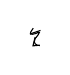
\begin{tikzpicture}[x=.4cm,y=.4cm,baseline=-.2ex]\draw (.12,.45) .. controls (-.04,.23) and (.01,.24) .. (.20,.28) .. controls (.34,.36) and (.36,.34) .. (.18,.12) .. controls (.10,-.03) and (.21,-.10) .. (.33,-.10);\draw (.02,.27)--(.35,.38);\draw (.18,.17)--(.11,-.11)--(.32,-.09);\end{tikzpicture}|\deleted{(}}}, on doit avoir un foncteur \deleted{\unsure{$V$|$Y$}} compatible avec ces structures \deleted{de} (cohomologie motivique)
\[
h:V\handwritten{\longrightarrow}\unsure{\rlap{\(\mathrm E\)}G|\mathbb{G}|G|E}\mathrm{rad}(M)\handwritten{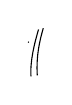
\begin{tikzpicture}[x=.4cm,y=.4cm,baseline=-.2ex]\draw (.08,-.75) .. controls (.04,-.20) and (.25,.50) .. (.32,.74);\draw (.28,-.72) .. controls (.24,-.10) and (.36,.40) .. (.47,.78);\fill (0,.34) circle (.025);\end{tikzpicture}}\quad\text{(structure de Koko sur }\mathrm{Grad}(M)\text{)}\handwritten{,}
\]
et on désire que les foncteurs cohomologiques habituels sur $V$ se factori\unsure{s\rlap{n}ant|s\rlap{r}ant|s\rlap{e}ant} par \deleted{$M$. Ceci impose}\inserted{des foncteurs sur $M$. On voudra\handwritten{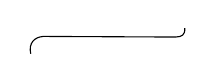
\begin{tikzpicture}[x=.4cm,y=.4cm,baseline=-.2ex]\draw (0,-.35) .. controls (-.08,.0) and (.13,.18) .. (.40,.20)--(4.6,.18) .. controls (4.80,.19) and (4.90,.24) .. (4.89,.46);\end{tikzpicture}}} que les foncteurs \deleted{fibres} obtenus sur $M$ so\rlap{n}i\unsure{\rlap{e}\rlap{t}n|\rlap{t}n}\rlap{t}nt des foncteurs fibres \deleted{\uline{tordus} seulement} véritables\inserted{\handwritten{(non tordus)}\handwritten{\begin{tikzpicture}[x=.4cm,y=.4cm,baseline=-.2ex]\draw (0,-.40) .. controls (.18,-.12) and (.28,.02) .. (.54,.07)--(2.70,.38) .. controls (2.86,.40) and (2.99,.45) .. (2.96,.63);\end{tikzpicture}}}, ce qui n'est pas idiot, \deleted{car}\inserted{\handwritten{\unsure{Car|car}}} on avait mis la structure de symétrie de Koko sur $\mathrm{Grad}(M)$: on s'est débarassé ainsi une fois pour toutes de la ``torsion''.

% source lines 12--15
On peut aussi, pour parler de vrais foncteurs fibres sur la catégorie des motifs semi-simples, remplacer la donnée de symmétrie ``géométrique'' i.e. de Koko pour le produit tensoriel dans \deleted{$\mathrm{Grad}(M)$}\inserted{la catégorie graduée $M$\handwritten{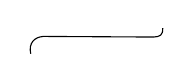
\begin{tikzpicture}[x=.4cm,y=.4cm,baseline=-.2ex]\draw (0,-.35) .. controls (-.08,.0) and (.13,.18) .. (.40,.20)--(3.9,.18) .. controls (4.10,.19) and (4.20,.24) .. (4.19,.46);\end{tikzpicture}}}, par la même canulée par le signe $(-1)^{ij}$ quand on a des \unsure{\rlap{r}a\rlap{a}r|$\mathbb{a}\mathbb{r}$}guments de degré $i,j$.

% source lines 16--24
11) Bien sûr, il y a lieu de chercher des théorèmes de structure intrinsèques, en termes de gerbes, pour des catégories $\unsure{\rlap{\(\mathrm N\)}C|\handwritten{\mathfrak{C}}|\handwritten{\mathscr{C}}|\mathbb{C}}$ munies des structures de 1º,\inserted{avec $k=\mathrm{End}(\underline{1})$ un corps donné.\handwritten{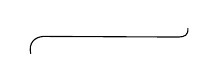
\begin{tikzpicture}[x=.4cm,y=.4cm,baseline=-.2ex]\draw (0,-.35) .. controls (-.08,.0) and (.13,.18) .. (.40,.20)--(4.7,.18) .. controls (4.90,.19) and (5.00,.24) .. (4.99,.46);\end{tikzpicture}}} Il y a lieu au besoin de supposer qu'il existe une extension de $k$ sur laquelle il y ait un foncteur fibre t\rlap{r}o\rlap{o}rdu gradué (ou m\unsure{\rlap{u}l|\rlap{b}l|b}tigradué ? Mais où s'arrêter ? ). Le plus beau serait évidemment de trouver un théorème de structure g\rlap{g}énéral, sans \uline{supposer} l'existence d'un foncteur fibre plus ou moins tordu où que ce soit, en définissant une notion assez générale de foncteur fibre tordu (?) et en \unsure{\rlap{r}p|p|$\mathbb{p}$}\rlap{r}p\unsure{\rlap{u}o|o}uv\rlap{q}ant qu'i\rlap{p}l y en a toujours sur une extension convenable de $k$.
